\documentclass[11.5pt, paper=a4]{article}

\usepackage[utf8]{inputenc}
\usepackage[english]{babel}
\usepackage[T1]{fontenc}

\usepackage{amsmath, amssymb, amscd, amsthm, amsfonts, mathtools}
\usepackage[left=2cm, right=2cm, top=1.5cm]{geometry}

\usepackage{graphicx}
\usepackage{graphicx}
\usepackage{hyperref}
\usepackage{physics}
\usepackage{tikz}
\usepackage{url}
\usepackage[square,numbers]{natbib} \usepackage{tabularx}
\usetikzlibrary{quantikz}

\usepackage{braket}
\usepackage{thmtools}
\usepackage{float}

%%% Theorem Style
\theoremstyle{definition}
\newtheorem{theorem}{Theorem}[section]
\newtheorem{definition}[theorem]{Definition}
\newtheorem{lemma}[theorem]{Lemma}
\newtheorem{conjecture}[theorem]{Conjecture}
\newtheorem{corollary}[theorem]{Corollary}

\numberwithin{theorem}{section}

%% Autoref prefixes
\renewcommand{\sectionautorefname}{Section}
\renewcommand{\subsectionautorefname}{Section}
\renewcommand{\subsubsectionautorefname}{Section}
\renewcommand{\figureautorefname}{Figure}
\def\theoremautorefname{Theorem}
\def\lemmaautorefname{Lemma}
\def\definitionautorefname{Definition}
\def\conjectureautorefname{Conjecture}
\def\algorithmautorefname{Algorithm}

%% Writing algorithms

\usepackage{algorithm} % captioning 
\usepackage{algpseudocode}
\usepackage{braket}
\usepackage{physics}
\usepackage{mathtools}
\usepackage{amsmath}
\usepackage[utf8]{inputenc}
% \def\NoNumber#1{{\def\alglinenumber##1{}\State #1}\addtocounter{ALG@line}{-1}}



\title{Quantum Algorithms, Spring 2022: Lecture 14 Scribe}

\author{Alapan Chaudhuri and Zeeshan Ahmed}

\date{\today}

\begin{document}

\maketitle

\section{Recap}

\subsection{Circuit for Quantum Fourier Transform}
\begin{figure*}[!htbp]
    \centering
    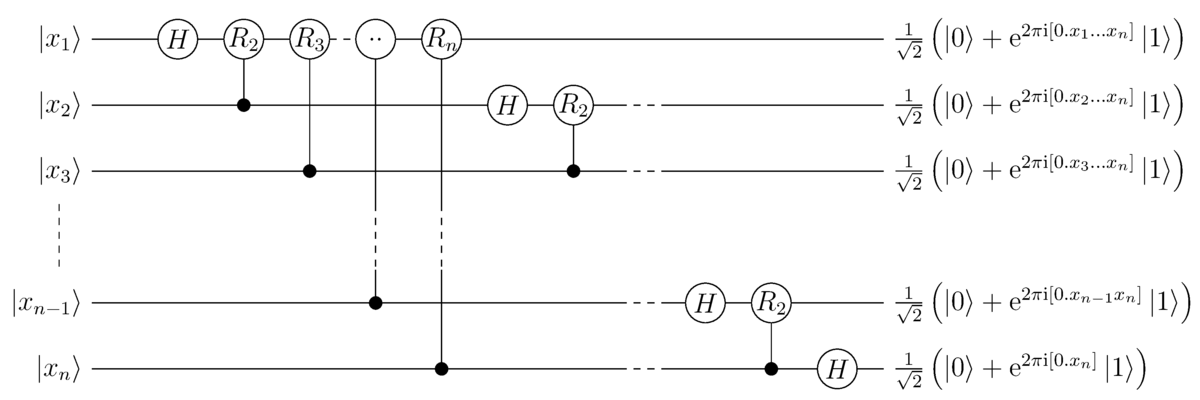
\includegraphics[width=\linewidth]{images/qft.png}
\end{figure*}

$$\text{QFT}(|x_{1}x_{2}\ldots x_{n}\rangle )={\frac {1}{\sqrt {N}}}\ \left(|0\rangle +e^{2\pi i\,[0.x_{n}]}|1\rangle \right)\otimes \left(|0\rangle +e^{2\pi i\,[0.x_{n-1}x_{n}]}|1\rangle \right)\otimes \cdots \otimes \left(|0\rangle +e^{2\pi i\,[0.x_{1}x_{2}\ldots x_{n}]}|1\rangle \right)$$

Here, we have $H$ and $R_m$ are the Hadamard and the controlled phase gates respectively.

$$H = \frac{1}{\sqrt 2} \begin{bmatrix}
1 & 1\\
1 & -1
\end{bmatrix}\ \ \ \ \ \ \ \ \ R_m = \begin{bmatrix}
1 & 0\\
0 & e^{2i\pi/2^m}
\end{bmatrix}$$

\subsection{Gate Complexity}
Implementation for Quantum Fourier Transform involves the above present circuit for QFT and $n/2$ - SWAP gates. Thus, the gate complexity of QFT is $O(n^2) = O(\log^2 N)$.

\section{Quantum Phase Estimation}
Suppose that $U$ is a unitary with a eigenvector $\ket{\phi}$ and eigenvalue $e^{2i\pi \theta},\ 0\leq \theta < 1$. If the cost of implementing $U$ is $T_u$, then given $\ket{\phi}$ we can obtain $\Tilde{\theta}$ such that $|\Tilde{\theta} - \theta| \leq \epsilon$ with success probability at least $1 - \dalta$ in time $T$ given by the following.

$$T = O\big(\frac{T_u}{\delta \epsilon}\big)$$

\subsection{Circuit for QPE}
The general quantum circuit for phase estimation is shown below. The top register contains $t$ 'counting' qubits, and the bottom contains qubits.
\begin{figure}[!htbp]
    \centering
    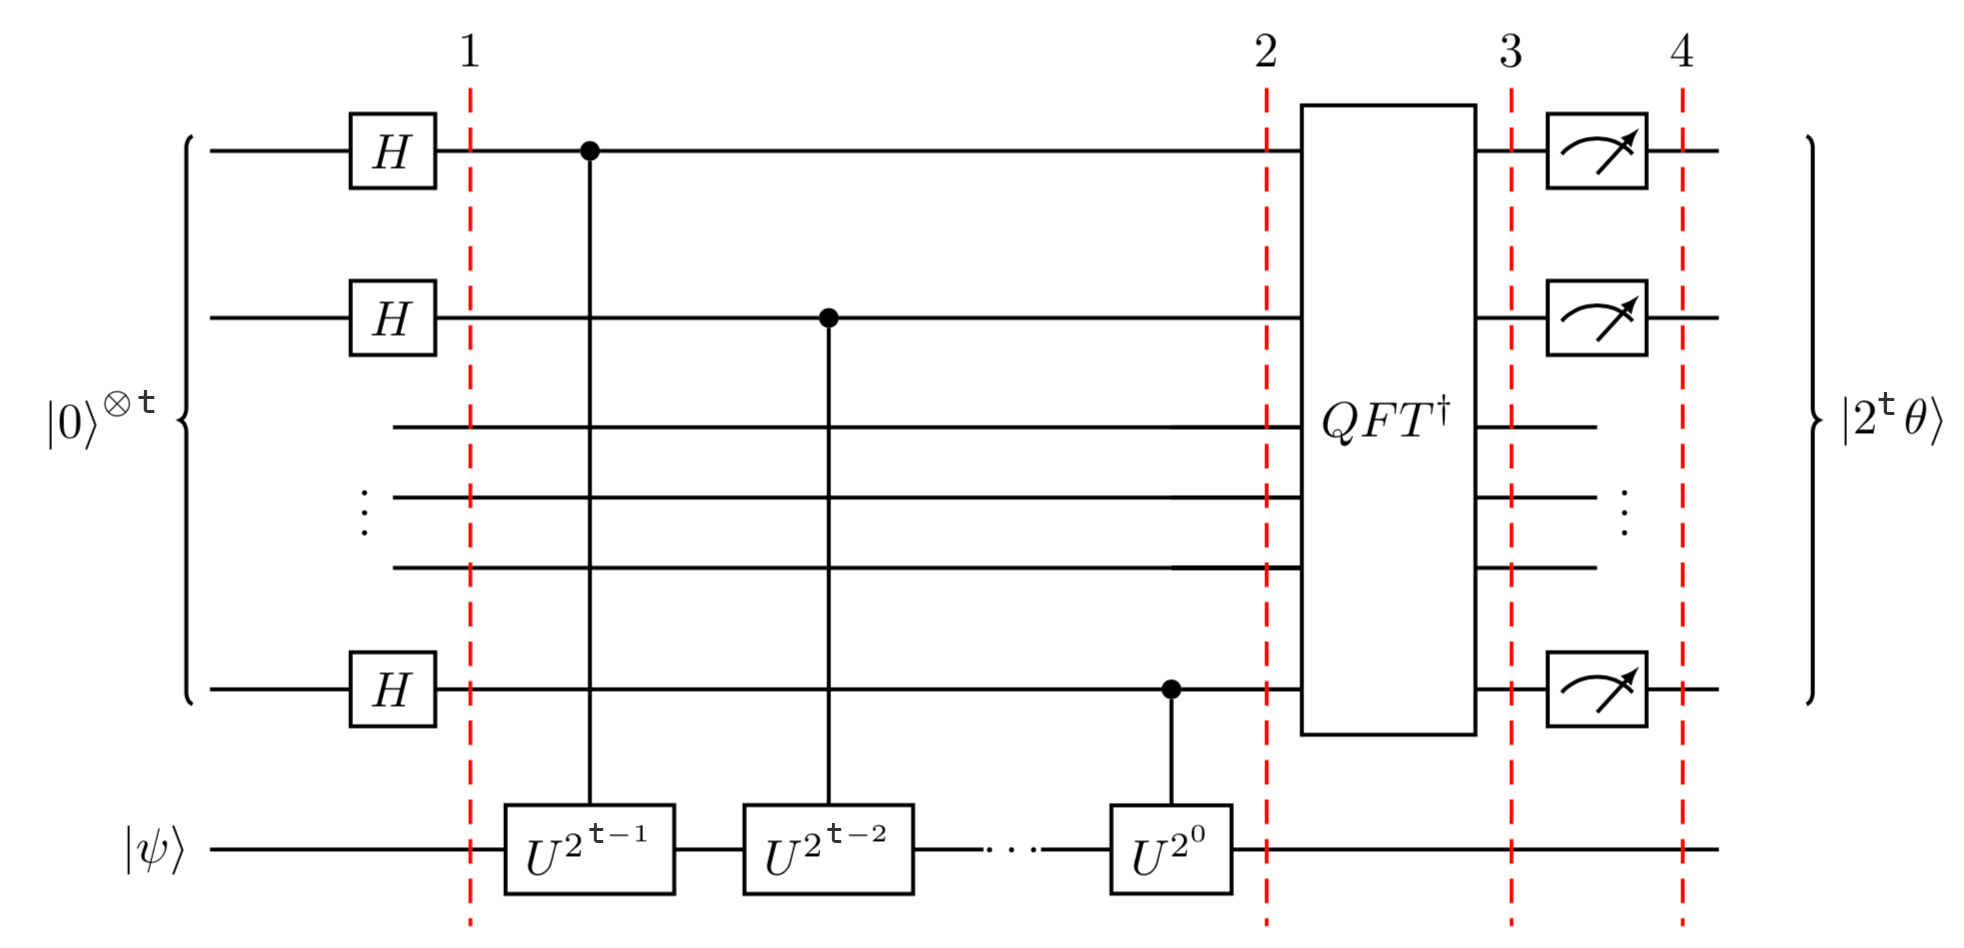
\includegraphics[width=\linewidth]{images/qpe.png}
    % \caption{Caption}
    % \label{fig:my_label}
\end{figure}

Now, $\lvert 0 \rangle^{\otimes t} \lvert \psi \rangle \xrightarrow{H^{\otimes t}\otimes I} {\frac {1}{\sqrt{2^{ t}}}}\left(|0\rangle +|1\rangle \right)^{\otimes t} \lvert \psi \rangle$. Also, $U^{2^{j}}|\psi \rangle =U^{2^{j}-1}U|\psi \rangle =U^{2^{j}-1}e^{2\pi i\theta }|\psi \rangle =\cdots =e^{2\pi i2^{j}\theta }|\psi \rangle$. Thus, upon applying the series of controlled unitaries we obtain the following.

$$\frac {1}{\sqrt{2 ^ t}} \left(|0\rangle+{e^{{2\pi i} \theta 2^{t-1}}}|1\rangle \right) \otimes \cdots \otimes \left(|0\rangle+{e^{{2\pi i} \theta 2^{1}}}\vert1\rangle \right) \otimes \left(|0\rangle+{e^{{2\pi i} \theta 2^{0}}}\vert1\rangle \right) \otimes |\psi\rangle = \frac{1}{\sqrt{2 ^ t}}\sum _{k=0}^{2^{t}-1}e^{{2\pi i} \theta k}|k\rangle \otimes \vert\psi\rangle$$

Furthermore, over the above expressed state QFT$^{\dagger}$ is applied resulting in the following expression.

$$\frac {1}{2^{\frac {t}{2}}}\sum _{k=0}^{2^{t}-1}e^{{2\pi i} \theta k}|k\rangle \otimes | \psi \rangle \xrightarrow{{QFT}_t^{\dagger}} \frac {1}{2^t}\sum _{x=0}^{2^{t}-1}\sum _{k=0}^{2^{t}-1} e^{-\frac{2\pi i k}{2^t}(x - 2^t \theta)} |x\rangle \otimes |\psi\rangle$$

Now, we can approximate the value of $\theta \in [0, 1]$ by rounding ${ 2^{t}\theta }$ to the nearest integer. This means that ${ 2^{t}\theta =a+2^{t}\delta ,}$ where ${ a}$ is the nearest integer to ${ 2^{t}\theta ,}$ and the difference ${ 2^{t}\delta }$ satisfies ${ 0\leqslant |2^{t}\delta |\leqslant {\tfrac {1}{2}}}$. Now, performing a measurement in the computational basis on the first register yields the result ${ |a\rangle }$ with probability $p_a$.

$${\begin{aligned} p_a&={\frac {1}{2^{2t}}}\left|{\frac {1-{e^{2\pi i2^{t}\delta }}}{1-{e^{2\pi i\delta }}}}\right|^{2}&&{\text{for }}\delta \neq 0\\[6pt]&={\frac {1}{2^{2t}}}\left|{\frac {2\sin \left(\pi 2^{t}\delta \right)}{2\sin(\pi \delta )}}\right|^{2}&& \text{given} \left|1-e^{2ix}\right|^{2}=4\left|\sin(x)\right|^{2}\\[6pt]&={\frac {1}{2^{2t}}}{\frac {\left|\sin \left(\pi 2^{t}\delta \right)\right|^{2}}{|\sin(\pi \delta )|^{2}}}\\[6pt]&\geqslant {\frac {1}{2^{2t}}}{\frac {\left|\sin \left(\pi 2^{t}\delta \right)\right|^{2}}{|\pi \delta |^{2}}}&&\text{given }|\sin(\pi \delta )|\leqslant |\pi \delta |{\text{ for }}|\delta |\leqslant {\frac {1}{2^{t+1}}}\\[6pt]\end{aligned}}$$

${\begin{aligned}\text{Thus, }p_a&\geqslant {\frac {1}{2^{2t}}}{\frac {|2\cdot 2^{t}\delta |^{2}}{|\pi \delta |^{2}}}\geqslant {\frac {4}{\pi ^{2}}}&&\text{given }|2\cdot 2^{t}\delta |\leqslant |\sin(\pi 2^{t}\delta )|{\text{ for }}|\delta |\leqslant {\frac {1}{2^{t+1}}}\\[6pt]\end{aligned}}$.

Now, we also know that $|\delta| < 1/2 \implies 0 < \pi |\delta| < 1/2 \implies \sin^2(\pi \delta) \geq 4 \delta^2$. This is because we have the inequality $|\sin x| \geq 2|x|/\pi, x \in [-\pi/2, \pi/2]$.

$$p_a = {\frac {1}{2^{2t}}}{\frac {\left|\sin \left(\pi 2^{t}\delta \right)\right|^{2}}{|\sin(\pi \delta )|^{2}}} < {\frac {1}{2^{2t}}}{\frac{1}{4\delta^2}}$$

Now, we are interested in all these $a$'s such that $|\delta| \geq \epsilon$. We will observe some $a \in [0, T - 1]$ and this will be satisfied by $\delta$ given as follows. Here, $T = 2^t$.

$$\delta = \begin{cases}\epsilon, \epsilon + 1/T, \epsilon + 2/T, \ldots\\
- \epsilon, -\epsilon - 1/T, -\epsilon - 2/T, \ldots\end{cases}$$

$$\text{Pr}[a: |\delta| \geq \epsilon] = \sum_{a: |\delta| \geq \epsilon} p_a \leq \frac{1}{4T^2}\left\{\sum_{k = 0}^\infty \frac{1}{\left(\epsilon + k/T\right)^2} + \sum_{k = 0}^\infty \frac{1}{\left(-\epsilon - k/T\right)^2}\right\} \leq \frac{1}{2T^2}\left\{\sum_{k = 0}^\infty \frac{1}{\left(\epsilon + k/T\right)^2}\right\} \leq \frac{1}{2} \sum_{k = 0}^\infty \frac{1}{(k + \epsilon T)^2}$$

$$\implies \text{Pr}[a: |\delta| \geq \epsilon] \leq \frac{1}{2} \sum_{k = 0}^\infty 1/k^2 \leq \frac{1}{2} \int_{\epsilon T}^{\infty} \frac{1}{x^2} dx \leq \frac{1}{2\epsilon T} < \frac{1}{\epsilon T}$$

Thus, we have $\text{Pr}[a: |\delta| \geq \epsilon] < \frac{1}{\epsilon T}$ and $\text{Pr}[|\theta - \Tilde{\theta}| < \epsilon] \geq 1 - \frac{1}{T\epsilon}$. So, we should have $\frac{1}{T\epsilon} < \delta \implies T > \frac{1}{T\epsilon} \implies t = 1 + \lceil \log_2{1/\delta} \rceil + \lceil \log_2{1/\epsilon} \rceil$, to have $|\theta  - \Tilde{\theta}| < \epsilon$ with prob $\geq 1 - \delta$.

\subsection{Complexity of QPE}
Now, cost of implementing $U = T_u$ whereas cost of implementing $c-U^{2^0}, c-U^{2^1}, \ldots, c-U^{2^{t - 1}} = O\left(T_u \sum_{j = 0}^{2^{t - 1}}2^j\right) = O\left(T_u 2^t\right) = O\left({T_u}/({\delta\epsilon})\right)$. However, we can improve this slightly by not adding ancilla qubits.
\begin{enumerate}
    \item Run QPE algorithm with 't' qubits in the first register $O\left(\log(1/\delta)\right)$ times.
    \item Compute the median of the outcomes and output the result.
    \item Thus, the new cost of implementation would be $O\left((T_u/\epsilon) \log(1/\delta)\right)$.
\end{enumerate}
\subsection{Remarks}
In some applications, we might be interested in preparing some specific eigenstates of $U$ and not care about the rest. In such cases QPE helps. These applications can be preparing ground states of Hamiltonian, Gibbs' state preparation, etc.

\nocite{*}
\bibliographystyle{plainnat}
\bibliography{references}
\end{document}